\section{Passive Meal-State Modeling}
\label{sec:meal-state-modeling}

\subsection{Motivation}
\label{subsec:meal-motivation}
AI-READI contains CGM, wearable signals, and static clinical descriptors, but not logged meals or carbohydrate doses \citep{aireadi2024}. The existing \texttt{predmeal\_flag} was therefore not a ground truth meal annotation, it is only a proxy scenario channel. The goal of this section is therefore narrower than simply asking whether “meal flags improve forecasting.” The real question is: can any deployable meal state representation add useful forecasting information beyond what the model already knows from current glucose level, recent glucose slope, and time of day? The pipeline is summarized in Fig.~\ref{fig:meal-pipeline} and Table~\ref{tab:meal-pipeline-summary}.

\begin{figure}[h!]
    \centering
    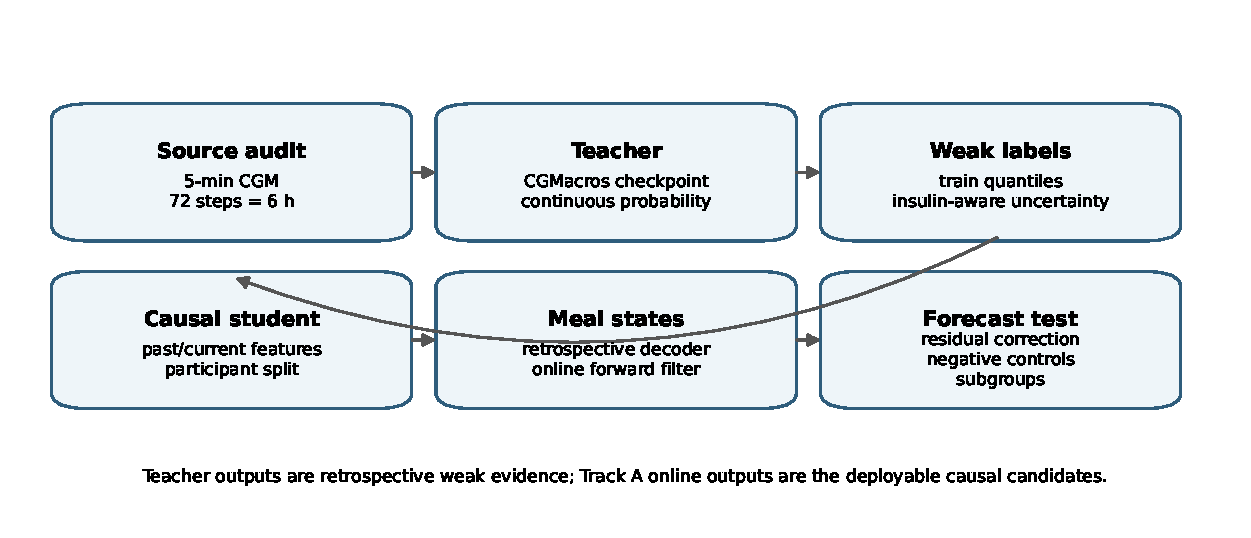
\includegraphics[width=\textwidth]{figures/meal_flags/meal_pipeline.pdf}
    \caption{Meal-flag improvement pipeline. The CGMacros teacher and the retrospective state decoder are diagnostic weak-supervision sources, the online Track A decoder and the causal student probability are the deployable candidates.}
    \label{fig:meal-pipeline}
\end{figure}
\begin{table}[h!]
    \centering
    \caption{Meal-transfer pipeline summary.}
    \label{tab:meal-pipeline-summary}
    \begin{tabular}{lr}
\toprule
Quantity & Value \\
\midrule
Participants & 1,591 \\
Rows & 4,015,355 \\
Teacher probability finite fraction & 0.993 \\
Corrected teacher flag rate & 0.114 \\
Surviving old binary artifact rate & 0.042 \\
Pseudo-label positives & 507,830 \\
Pseudo-label negatives & 1,085,414 \\
Pseudo-label uncertain & 2,422,111 \\
Causal student validation AP & 0.863 \\
Causal student validation AUC & 0.928 \\
Retrospective decoded events & 53,024 \\
Retrospective decoded flag rate & 0.290 \\
Online prefix invariance max absolute difference & 0.000 \\
Online response-size validation macro-F1 & 0.767 \\
Independent evaluation events & 77,835 \\
\bottomrule
\end{tabular}

\end{table}

\subsection{Transfer of the CGMacros meal detector}
\label{subsec:meal-transfer-teacher}
The original meal detector transferred from CGMacros uses a dilated CNN followed by a two-layer bidirectional LSTM. It processes 6 hour CGM windows sampled every five minutes. Because the LSTM is bidirectional, the prediction at a given anchor can depend on CGM values after that anchor. However, if the detector can read future glucose, then it can identify the rise caused by a meal after the rise has already begun. That makes it useful as a retrospective diagnostic, but not as a deployable meal signal available at time (t). It also means that any forecasting gain from this bidirectional teacher may come from future glucose leakage rather than from true meal anticipation.

For this reason, the bidirectional teacher is not treated as a valid causal input. It is kept as a leakage diagnostic: it shows how much performance can be obtained when future glucose is accidentally allowed into the feature

\subsection{Correction of the AI-READI meal flag model}
\label{subsec:meal-reconstruction}
The original downstream artifact kept only a thresholded binary flag and discarded the teacher's continuous probability. Reconstructing overlap-averaged probabilities recovered finite values for 99.3\% of rows and a corrected teacher flag rate of 0.114, compared with 0.042 for the surviving old binary artifact. The reconstruction is a faithful recovery of the source signal, but the source signal is itself bidirectional, so neither the corrected probability nor the surviving \texttt{predmeal\_flag} is causal. Figure~\ref{fig:meal-teacher-reconstruction} shows the information loss of the old artifact.

\begin{figure}[h!]
    \centering
    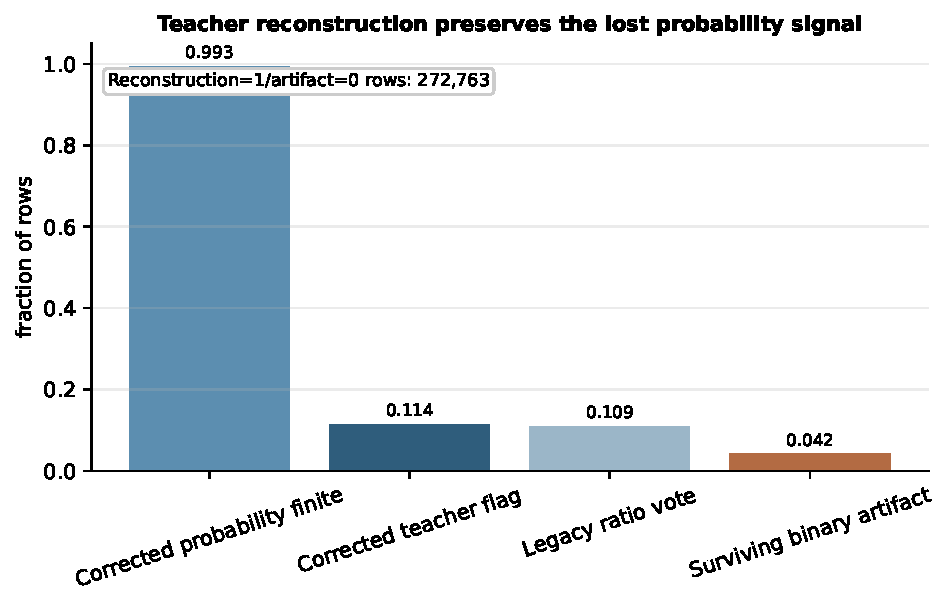
\includegraphics[width=0.82\textwidth]{figures/meal_flags/teacher_reconstruction.pdf}
    \caption{Corrected teacher reconstruction. The continuous teacher probability is available for nearly all rows, while the old binary artifact is merge-diluted.}
    \label{fig:meal-teacher-reconstruction}
\end{figure}

\subsection{Weak Target-Domain Supervision}
\label{subsec:meal-weak-supervision}
Weak labels were constructed from the AI-READI training split using data-driven glucose-response quantiles rather than fixed glucose thresholds. This avoids imposing one universal meal-response definition across participants with very different glycemic profiles.

Two changes make the supervision more cautious. First, insulin users are excluded from meal-label training because a meal-like glucose pattern in an insulin-treated participant may reflect unobserved insulin timing rather than food intake. These rows are not discarded from the analysis entirely, but they are treated as lower-confidence metabolic events.

Second, uncertain rows are not simply dropped. Some uncertain windows may correspond to early pre-rise periods, which are precisely the moments where a meal detector could be useful for forecasting. These rows are therefore assigned a soft onset-distance target when appropriate. This allows the model to learn from gradual transitions instead of only from obvious post-meal rises.

The response-size label should also be interpreted carefully. It measures the realized glucose excursion after an event. It is not a carbohydrate amount and should not be described as a meal dose.

\subsection{Causal student model}
\label{subsec:meal-causal-student}
The causal student is trained using only information available at or before the current time: past and current CGM, wearable signals, clock features, and static participant context. Teacher outputs and future glucose are used only to construct weak labels; they are not provided to the student at inference. The student performs well as a pseudo label model, but that is not enough to prove it is useful for forecasting. A high AUC or average precision only shows that the student can reproduce the weak labels. The more important test is whether the student adds forecasting information beyond glucose slope, glucose level, and time of day. For this reason, the student is evaluated through the forecasting gate rather than judged only by classification metrics.

\subsection{Retrospective and Online Meal-State Decoding}
\label{subsec:meal-decoders}
The student probability is converted into structured meal states. The retrospective decoder identifies onset, rising, peak, and recovery phases using information from the full segment, so it is useful for event discovery and interpretation. The online decoder, in contrast, runs strictly forward in time and is the deployable version.

The decoded response-size categories are physiologically ordered: larger decoded events correspond to larger mean peak glucose rises. This supports the idea that the decoder is capturing real glucose-response structure. However, the retrospective decoder is still not deployable because it uses full segment information. Only the online filter can be considered a causal candidate.
Examples appear in Fig.~\ref{fig:meal-state-examples}.

\begin{figure}[h!]
    \centering
    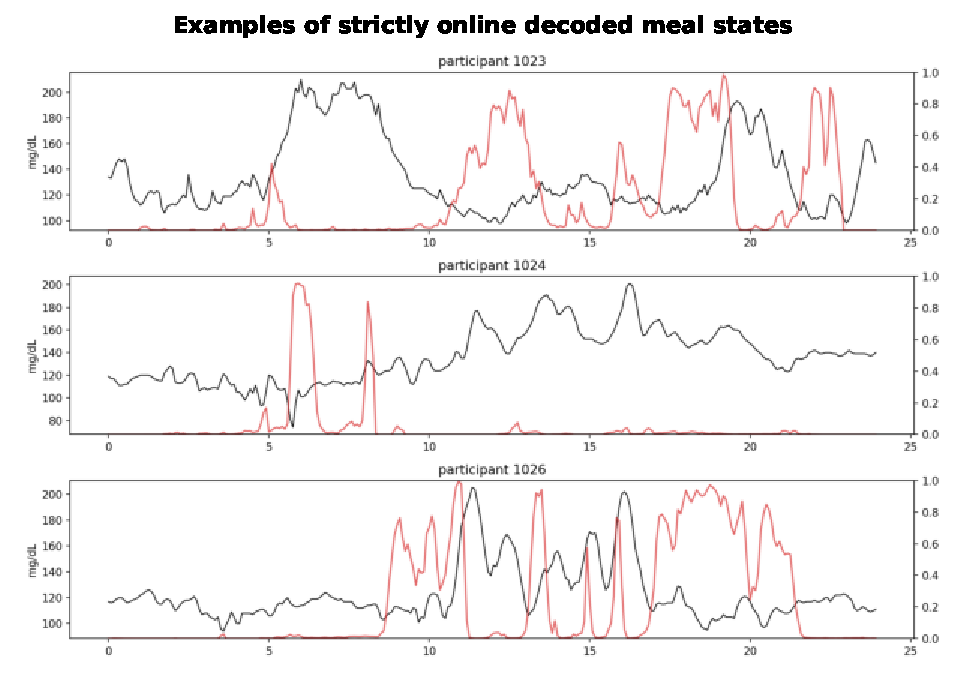
\includegraphics[width=\textwidth]{figures/meal_flags/state_examples.pdf}
    \caption{Strictly online decoded meal-state examples. State changes are produced by a forward recursion and do not use future glucose, future wearables, or teacher outputs at inference.}
    \label{fig:meal-state-examples}
\end{figure}

\subsection{Experimental Feature Representations}
\label{subsec:meal-feature-representations}

All meal representations are evaluated in the same residual-correction framework. The pretrained SSMCGM-Stream median forecast is kept as the base forecast, and each candidate meal feature is allowed to add a correction to that base prediction. The \texttt{q50} median from the
pretrained SSMCGM-Stream model is used as a base forecast, and each candidate meal
representation $M_t^{(m)}$ is evaluated as an additive residual correction:
\begin{equation}
    \widehat{y}_{t+h}^{(m)}
    = \widehat{y}_{t+h}^{q50}
    + r_m\!\left(X_t^{\mathrm{base}},\,M_t^{(m)},\,h\right),
    \label{eq:meal-residual-framework}
\end{equation}
where the baseline feature vector is
\begin{equation}
    X_t^{\mathrm{base}}
    = \left[G_t,\;\Delta G_{15,t},\;\Delta G_{30,t},\;\Delta G_{60,t},\;
      \sin\theta_t,\;\cos\theta_t\right],\quad
    \theta_t = \tfrac{2\pi m_t}{1440}.
    \label{eq:meal-base-features}
\end{equation}
Here $G_t$ is the current glucose reading, $\Delta G_{\tau,t}$ are $\tau$-minute backward
slopes, and $(\sin\theta_t, \cos\theta_t)$ encode time of day continuously.

The retrospective setups build on this with increasingly rich leakage diagnostics:
\begin{equation}
    \underbrace{X_t^{\mathrm{base}}}_{A'}
    \;\longrightarrow\;
    \underbrace{\bigl[X_t^{\mathrm{base}},\,B_t\bigr]}_{B}
    \;\longrightarrow\;
    \underbrace{\bigl[X_t^{\mathrm{base}},\,\bar{p}_t^T\bigr]}_{C}.
    \label{eq:meal-retro-chain}
\end{equation}
The leakage-free chain replaces retrospective signals with causal ones:
\begin{equation}
    \underbrace{X_t^{\mathrm{base}}}_{A'}
    \;\longrightarrow\;
    \underbrace{\bigl[X_t^{\mathrm{base}},\,p_t^{T,\mathrm{causal}}\bigr]}_{C'}
    \;\longrightarrow\;
    \underbrace{\bigl[X_t^{\mathrm{base}},\,\widehat{p}_t^S\bigr]}_{D}
    \;\longrightarrow\;
    \underbrace{\bigl[X_t^{\mathrm{base}},\,\widehat{p}_t^S,\,\boldsymbol{\alpha}_t,\,\tau_t,\,c_t,\,\mathbf{q}_t\bigr]}_{H}.
    \label{eq:meal-causal-chain}
\end{equation}
The central empirical finding is:
\begin{equation}
    C \;\gg\; C' \;\approx\; D \;\approx\; H \;\approx\; A'.
    \label{eq:meal-central-comparison}
\end{equation}
The large performance advantage of C disappears when future-glucose access is removed; the
causal teacher, student, and online state carry little forecasting information beyond what
glucose level, slope, and clock already provide.

Table~\ref{tab:meal-setup-definitions} gives the formal definition of each setup's added
information, its mathematical representation, and its role in the evaluation.

\begin{table}[h!]
\centering
\footnotesize
\renewcommand{\arraystretch}{1.35}
\caption{Formal definitions of the seven evaluation setups. ``Future info?'' marks setups
that use glucose or wearable data after time $t$ when computing the meal feature value.
These setups are diagnostic only and are not deployable.}
\label{tab:meal-setup-definitions}
\setlength{\tabcolsep}{4pt}
\begin{tabular}{@{}l p{3.8cm} p{4.0cm} p{3.2cm} c@{}}
\toprule
Setup & Information added to $X_t^{\mathrm{base}}$ & Meal representation $M_t^{(m)}$ & Role & Future? \\
\midrule
\textbf{q50}
  & None. Original SSMCGM-Stream median used directly.
  & $\widehat{y}_{t+h}^{q50}$ (no correction applied)
  & End-to-end baseline before any residual correction.
  & No \\[2pt]

\textbf{A$'$}
  & Current glucose $G_t$, three backward slopes $\Delta G_{\tau,t}$, clock $(\sin,\cos)\theta_t$.
  & $X_t^{\mathrm{base}}$ per Eq.~\eqref{eq:meal-base-features}
  & Fair harness baseline; isolates how much error slope and clock already explain.
  & No \\[2pt]

\textbf{B}
  & Thresholded binary predmeal flag from the bidirectional teacher: $B_t = \mathbb{1}\!\left[\bar{p}_t^T > \tau\right]$.
  & $\bigl[X_t^{\mathrm{base}},\,B_t\bigr]$
  & Leakage diagnostic for the old binary representation; retrospective.
  & Yes \\[2pt]

\textbf{C}
  & Corrected continuous teacher probability $\bar{p}_t^T = \frac{1}{|\mathcal{W}_t|}\sum_{w\in\mathcal{W}_t}p_{t,w}^T$.
  & $\bigl[X_t^{\mathrm{base}},\,\bar{p}_t^T\bigr]$
  & Retrospective oracle ceiling. Strong performance reflects future-glucose leakage, not deployable signal.
  & Yes \\[2pt]

\textbf{C$'$}
  & Causal teacher score computed from $G_{\le t}$ only: $p_t^{T,\mathrm{causal}} = f_\theta^T(G_{\le t})$.
  & $\bigl[X_t^{\mathrm{base}},\,p_t^{T,\mathrm{causal}}\bigr]$
  & Leakage-free teacher ceiling. Gap $C \gg C'$ quantifies how much of C's gain was unreachable future leakage.
  & No \\[2pt]

\textbf{D}
  & Causal student probability $\widehat{p}_t^S = f_\phi(X_{\le t}^{\mathrm{CGM}}, W_{\le t}, S_i)$, using past/current CGM, wearables, clock, and static context.
  & $\bigl[X_t^{\mathrm{base}},\,\widehat{p}_t^S\bigr]$
  & Basic deployable meal representation; tests whether the student adds signal beyond $A'$.
  & No \\[2pt]

\textbf{H}
  & Full online state: student probability plus structured phase decoder outputs $(\boldsymbol{\alpha}_t, \tau_t, c_t, \mathbf{q}_t)$, where $\boldsymbol{\alpha}_t$ is the online phase distribution (none/onset/rising/peak/recovery), $\tau_t$ is time since onset, $c_t$ is confidence, $\mathbf{q}_t$ is response-size probability.
  & $\bigl[X_t^{\mathrm{base}},\,\widehat{p}_t^S,\,\boldsymbol{\alpha}_t,\,\tau_t,\,c_t,\,\mathbf{q}_t\bigr]$
  & Richest deployable representation; adds temporal organization to D, but incremental gain is small when components correlate with slope already in $X_t^{\mathrm{base}}$.
  & No \\
\bottomrule
\end{tabular}
\end{table}

\subsection{Forecasting Evaluation and Selection Gate}
\label{subsec:meal-forecasting-evaluation}
Meal features were evaluated as residual corrections on top of the cached 60-minute SSMCGM-Stream \texttt{q50} forecast,
\begin{equation}
    \yhat^{(m)}_{i,t+h} = \yhat^{q50}_{i,t+h} + r_m(C_{i,t}, M^{(m)}_{i,t}, h),
    \label{eq:meal-residual-correction}
\end{equation}
fit on the validation cache and evaluated on the participant-disjoint test cache. Alignment passed on 1,660,377 test rows with maximum target residual 0.500 mg/dL and same-segment fraction 1.000.

Whole-horizon MAE60 is not the gate. A 60-minute average washes out the post-prandial excursion, and the negative controls below confirm almost no timing-specific signal exists on that endpoint. The gate is re-anchored on the endpoints where a meal acts, meal-window MAE, one hour peak error, time to peak, hyperglycemia AUPRC, and recall at precision 0.80 for the event \(\max(y \text{ over the next hour}) > 180\) mg/dL. A feature is selected only if, on the non-insulin cohort, it improves at least two of these endpoints over the baseline and beats shuffled, time-shifted, and block-shuffled controls with a participant-bootstrap interval that excludes zero. The decision is computed in code, not asserted in prose.

The baseline is A', a within-harness residual model on CGM slope, level, and clock only. The harness cost of A' relative to untouched \texttt{q50} is small on the non-insulin cohort, -0.005 mg/dL on MAE60 and -0.344 mg/dL on peak error, so meal comparisons are made against A' rather than against \texttt{q50} to separate the harness penalty from feature value. A' already captures most of the recoverable post-prandial signal, reaching meal-window MAE 13.745 and peak error 10.549 versus 13.856 and 10.893 for \texttt{q50}.

\begin{table}[h!]
    \centering
    \caption{Reachable ceiling and leakage diagnostics on the non-insulin cohort. A' is the slope and clock baseline, C' is the leakage-free causal teacher ceiling, C and B are bidirectional-teacher leakage diagnostics. Lower is better for MAE, peak, and time to peak, higher is better for AUPRC and recall.}
    \label{tab:meal-main-results}
    \resizebox{\textwidth}{!}{%
\begin{tabular}{lrrrrrr}
\toprule
Setup & Meal MAE & Peak err. & TTP err. & Hyper AUPRC & Recall@.80 & MAE60 \\
\midrule
q50 & 13.856 & 10.893 & 19.4 & 0.876 & 0.776 & 14.357 \\
A$'$: slope+level+clock & 13.745 & 10.549 & 20.1 & 0.876 & 0.776 & 14.351 \\
C$'$: causal teacher (ceiling) & 13.724 & 10.542 & 20.0 & 0.876 & 0.778 & 14.333 \\
C: bidir teacher (leakage) & 11.286 & 8.150 & 17.5 & 0.926 & 0.862 & 11.789 \\
B: predmeal flag (leakage) & 13.226 & 9.876 & 19.7 & 0.888 & 0.792 & 13.737 \\
\bottomrule
\end{tabular}
}

\end{table}

The leakage-free causal teacher C' is the reachable ceiling, and it sits essentially at A', meal-window MAE 13.724 and peak error 10.542. The old bidirectional teacher C reaches meal-window MAE 11.286 and peak error 8.150, but that gap is leakage, because the only difference between C and C' is whether the teacher window is allowed to read future glucose. The previously reported gain from C, from 14.846 to 12.460 on MAE60, was therefore an oracle effect rather than reachable headroom. The deployable features cluster at A', the student probability D reaching meal-window MAE 13.711 and peak error 10.541, and the online full state H reaching 13.710 and 10.523.

\begin{table}[h!]
    \centering
    \caption{Deployable causal representations against A' on the gate endpoints.}
    \label{tab:meal-causal-results}
    \resizebox{\textwidth}{!}{%
\begin{tabular}{lrrrrrr}
\toprule
Setup & Meal MAE & Peak err. & TTP err. & Hyper AUPRC & Recall@.80 & MAE60 \\
\midrule
A$'$: slope+level+clock & 13.745 & 10.549 & 20.1 & 0.876 & 0.776 & 14.351 \\
C$'$: causal teacher (ceiling) & 13.724 & 10.542 & 20.0 & 0.876 & 0.778 & 14.333 \\
D: student prob. & 13.711 & 10.541 & 19.7 & 0.877 & 0.777 & 14.266 \\
G: online state & 13.712 & 10.524 & 19.7 & 0.877 & 0.776 & 14.268 \\
H: online full state & 13.710 & 10.523 & 19.7 & 0.877 & 0.776 & 14.263 \\
\bottomrule
\end{tabular}
}

\end{table}

The orthogonalization test explains the clustering. After regressing each feature on slope, level, and clock, the leakage-free causal teacher C' has partial correlation 0.027 with the \texttt{q50} residual, the student probability D has 0.147, while the bidirectional teacher C has 0.519. The large orthogonal signal belongs only to the leaky features, so the deployable features carry little information that the CGM slope does not already provide.

\begin{table}[h!]
    \centering
    \caption{Partial-information test against the CGM slope. Partial correlation with the q50 residual after removing slope, level, and clock, and the change in gate endpoints from adding the orthogonalized feature to the slope-only model.}
    \label{tab:meal-partial-information}
    \resizebox{\textwidth}{!}{%
\begin{tabular}{llrrr}
\toprule
Setup & Feature & Partial corr. & $\Delta$ Meal MAE & $\Delta$ Peak \\
\midrule
B: predmeal flag (leakage) & predmeal\_flag & 0.278 & 0.498 & 0.673 \\
C$'$: causal teacher (ceiling) & cgmacros\_teacher\_probability\_causal & 0.027 & 0.019 & 0.001 \\
C: bidir teacher (leakage) & cgmacros\_teacher\_probability & 0.519 & 2.302 & 2.385 \\
D: student prob. & student\_meal\_probability & 0.147 & 0.025 & 0.008 \\
G: online state & student\_meal\_probability & 0.147 & 0.025 & 0.008 \\
H: online full state & student\_meal\_probability & 0.147 & 0.025 & 0.008 \\
\bottomrule
\end{tabular}
}

\end{table}

\subsection{Leakage Audits and Negative Controls}
\label{subsec:meal-leakage-controls}
The leakage audit records the maximum future input offset used by each feature. The student probability and online states have zero future offset, so they are leakage-free. The original \texttt{predmeal\_flag} and legacy bidirectional teacher have a positive future offset, meaning they can read glucose after the anchor time.
\begin{table}[h!]
    \centering
    \caption{Feature provenance and leakage audit. A positive input offset means the feature can read CGM later than its anchor.}
    \label{tab:meal-feature-provenance}
    \resizebox{\textwidth}{!}{%
\begin{tabular}{lrll}
\toprule
Feature & Max input offset (steps) & Uses future glucose & Leakage free \\
\midrule
student\_meal\_probability & 0 & False & True \\
online\_state\_features & 0 & False & True \\
predmeal\_flag & 71 & True & False \\
cgmacros\_teacher\_probability (legacy\_bidirectional) & 71 & True & False \\
cgmacros\_teacher\_probability\_causal (teacher\_mode=causal) & 0 & False & True \\
\bottomrule
\end{tabular}
}

\end{table}

The negative controls are the key evidence for whether a feature carries timing-specific information. A real meal feature should perform better at its true timing than when it is shuffled, shifted, or block-shuffled within participant. (Fig.~\ref{fig:meal-negative-controls}). For the deployable student probability, the real versus control gap is small. This means the feature timing does not add much beyond the baseline glucose trajectory. The leaky \texttt{predmeal\_flag} B shows a large real versus control gap, which is consistent with the leakage analysis:  the feature looks strongly predictive because it is partially informed by future glucose.

\begin{table}[h!]
    \centering
    \caption{Meal-state negative controls on the gate endpoints. Real timing versus shuffled, shifted, and block-shuffled meal features.}
    \label{tab:meal-negative-controls}
    \resizebox{\textwidth}{!}{%
\begin{tabular}{llrrr}
\toprule
Setup & Control & Meal MAE & Peak err. & Hyper AUPRC \\
\midrule
C$'$: causal teacher (ceiling) & real & 13.724 & 10.542 & 0.876 \\
C$'$: causal teacher (ceiling) & shuffle & 13.830 & 10.492 & 0.876 \\
C$'$: causal teacher (ceiling) & time\_shift & 13.859 & 10.716 & 0.874 \\
C$'$: causal teacher (ceiling) & block\_shuffle & 13.824 & 10.521 & 0.875 \\
D: student prob. & real & 13.711 & 10.541 & 0.877 \\
D: student prob. & shuffle & 13.792 & 10.601 & 0.876 \\
D: student prob. & time\_shift & 13.741 & 10.541 & 0.876 \\
D: student prob. & block\_shuffle & 13.813 & 10.500 & 0.876 \\
H: online full state & real & 13.710 & 10.523 & 0.877 \\
H: online full state & shuffle & 13.819 & 10.554 & 0.876 \\
H: online full state & time\_shift & 17.159 & 16.906 & 0.757 \\
H: online full state & block\_shuffle & 13.834 & 10.468 & 0.876 \\
B: predmeal flag (leakage) & real & 13.226 & 9.876 & 0.888 \\
B: predmeal flag (leakage) & shuffle & 14.116 & 14.174 & 0.866 \\
B: predmeal flag (leakage) & time\_shift & 13.714 & 10.689 & 0.868 \\
B: predmeal flag (leakage) & block\_shuffle & 14.206 & 12.196 & 0.871 \\
\bottomrule
\end{tabular}
}

\end{table}

\begin{figure}[h!]
    \centering
    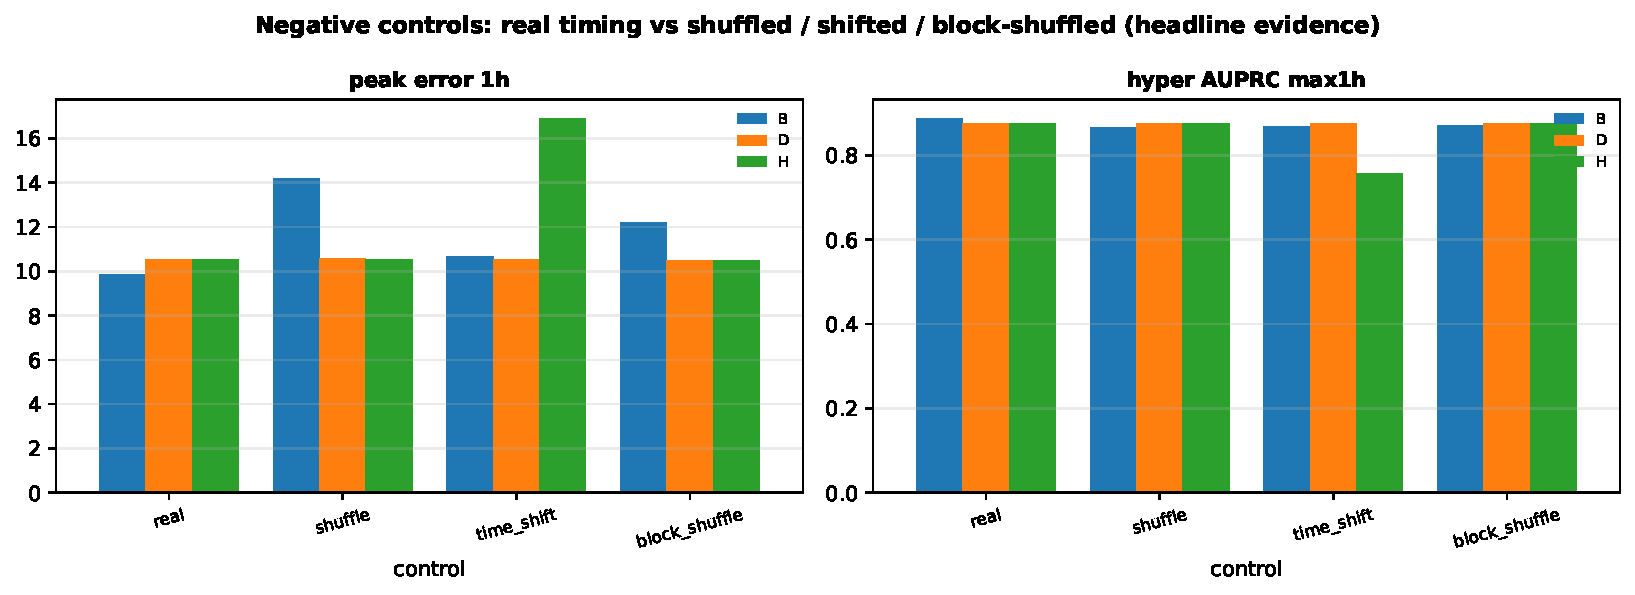
\includegraphics[width=\textwidth]{figures/meal_flags/negative_controls.pdf}
    \caption{Negative controls are the central evidence. The real-versus-control gap is the only honest measure of timing-specific meal signal, and it is small for the deployable features on the gate endpoints.}
    \label{fig:meal-negative-controls}
\end{figure}

\begin{table}[h!]
    \centering
    \caption{Coded selection decision on the non-insulin cohort. A feature is selected only if it is leakage free and passes at least two gate endpoints against A' with controls beaten.}
    \label{tab:meal-selection}
    \begin{tabular}{lrll}
\toprule
Setup & Passing endpoints & Leakage free & Selected \\
\midrule
B: predmeal flag (leakage) & 5/2 & False & \textbf{False} \\
C$'$: causal teacher (ceiling) & 1/2 & True & \textbf{False} \\
C: bidir teacher (leakage) & 5/2 & False & \textbf{False} \\
D: student prob. & 1/2 & True & \textbf{False} \\
G: online state & 2/2 & True & \textbf{True} \\
H: online full state & 2/2 & True & \textbf{True} \\
\bottomrule
\end{tabular}

\end{table}
Therefore, for non insulin participants, the online meal states can be described as weak but controlled forecasting features. In insulin users, they should be reported as low-confidence meal like metabolic events rather than literal meal detections.
\subsection{Subgroup and Insulin Sensitivity Analyses}
\label{subsec:meal-subgroups}
Insulin users are analyzed separately because AI-READI does not provide insulin timing or dose. Without those variables, many meal-like glucose responses in insulin-treated participants may actually reflect unobserved insulin dynamics.
In the non-insulin cohort, the online full state (H) gives a small improvement over (A') on peak error and MAE60. The effect is present but modest. In insulin users, the error is larger and the uncertainty is wider, and the same comparison is not clearly favorable.
\begin{table}[h!]
    \centering
    \caption{Subgroup results split by insulin status for A', the online full state H, and the student probability D.}
    \label{tab:meal-subgroup-results}
    \resizebox{\textwidth}{!}{%
\begin{tabular}{llrrrr}
\toprule
Insulin & Setup & $n$ & Meal MAE & Peak err. & MAE60 \\
\midrule
med\_insulin=0 & q50 & 200 & 13.856 & 10.893 & 14.357 \\
med\_insulin=1 & q50 & 16 & 16.745 & 13.733 & 20.660 \\
med\_insulin=0 & A$'$: slope+level+clock & 200 & 13.745 & 10.549 & 14.351 \\
med\_insulin=1 & A$'$: slope+level+clock & 16 & 16.560 & 13.456 & 20.805 \\
med\_insulin=0 & D: student prob. & 200 & 13.711 & 10.541 & 14.266 \\
med\_insulin=1 & D: student prob. & 16 & 16.698 & 13.528 & 21.059 \\
med\_insulin=0 & H: online full state & 200 & 13.710 & 10.523 & 14.263 \\
med\_insulin=1 & H: online full state & 16 & 16.629 & 13.508 & 20.704 \\
\bottomrule
\end{tabular}
}

\end{table}

\begin{figure}[h!]
    \centering
    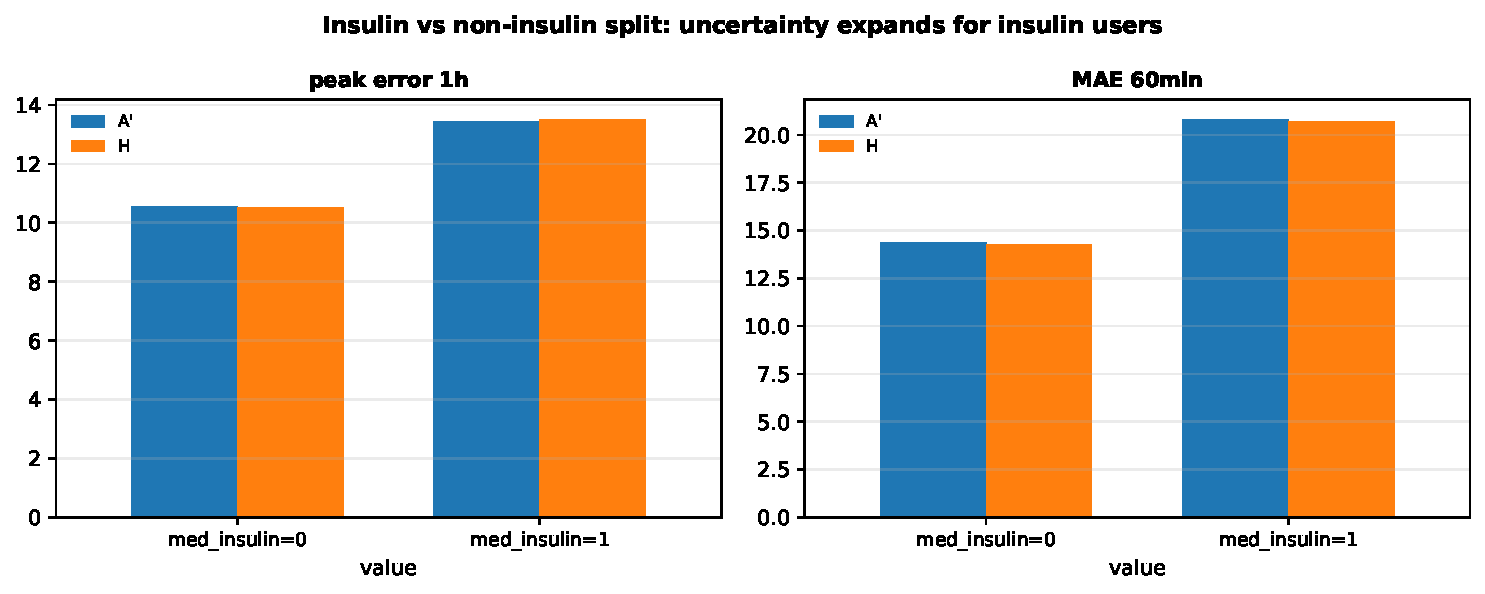
\includegraphics[width=\textwidth]{figures/meal_flags/insulin_sensitivity.pdf}
    \caption{Insulin versus non-insulin split. The non-insulin story is clean, while uncertainty expands for insulin users.}
    \label{fig:meal-insulin-sensitivity}
\end{figure}

\subsection{Discussion and Limitations}
\label{subsec:meal-discussion-limitations}
The coded gate selects the online state representations (G) and (H) on the non-insulin cohort, mainly because they improve meal-window MAE and hyperglycemia AUPRC. However, the effect sizes are small: the improvement is on the order of a few hundredths of a mg/dL for meal-window MAE and a few thousandths for AUPRC. The one-hour peak-error improvement does not survive all negative controls.

The strongest conclusion is therefore not that meal states strongly improve forecasting. The stronger and more rigorous conclusion is that the original large meal-feature gain was mostly caused by future-glucose leakage. Once the meal pathway is made causal, most of the apparent advantage disappears because the remaining information overlaps with current glucose slope and time of day.

At this stage, the meal-state branch is best described as a validated weak-supervision and diagnostic pathway. It is not yet strong enough to justify full SSMCGM retraining as a production meal representation. A future feature would need to provide earlier information that is not already contained in the CGM slope

\begin{figure}[h!]
    \centering
    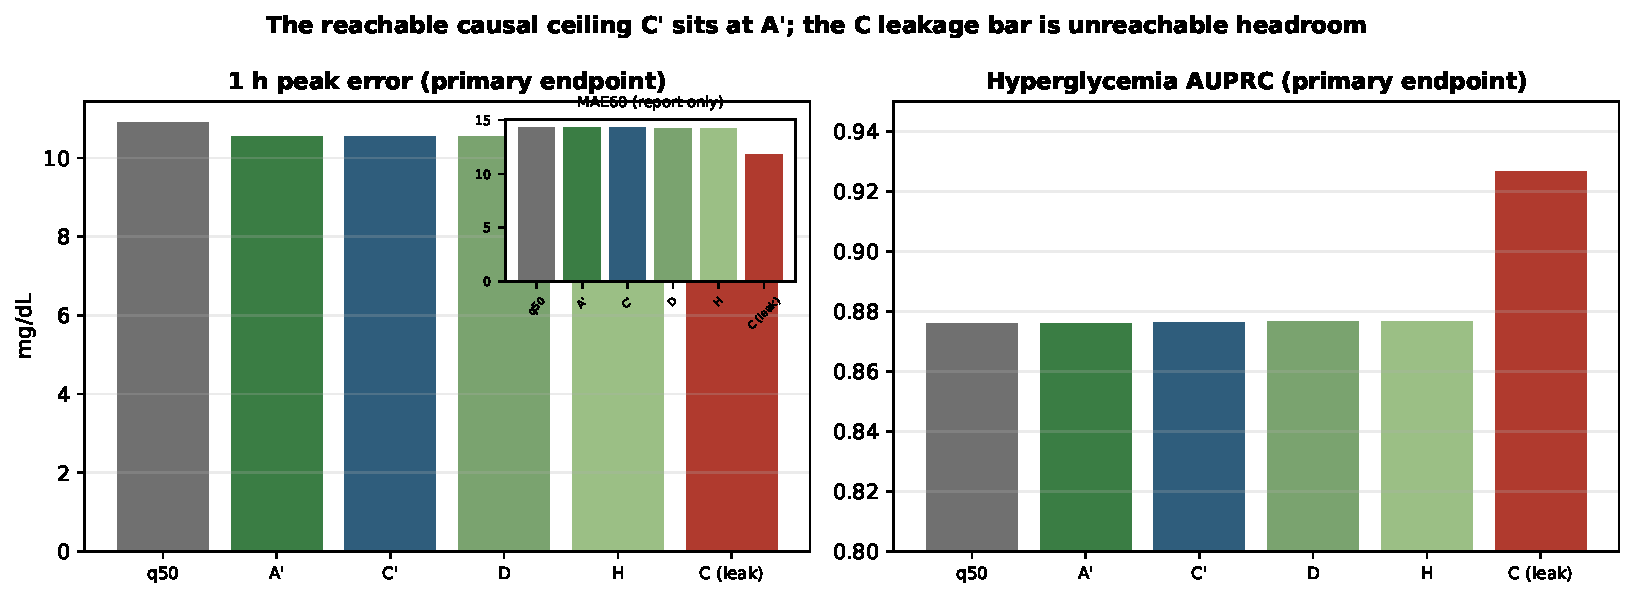
\includegraphics[width=\textwidth]{figures/meal_flags/retrospective_causal_gap.pdf}
    \caption{Peak error and hyperglycemia AUPRC are the primary axes, with MAE60 demoted to the inset. The reachable causal ceiling C' sits at A', while the C leakage bar is unreachable headroom.}
    \label{fig:meal-retrospective-causal-gap}
\end{figure}

At the current checkpoint the meal-state branch is a validated weak-supervision and diagnostic pathway, not a selected production meal representation for SSMCGM retraining. The next step that could change the decision is a label that carries pre-rise information the CGM slope lacks, evaluated with the same coded gate.

\subsection{Pre-Rise Wearable Detector}
\label{subsec:prerise-wearable-detector}

To evaluate whether wearable signals can provide the missing lead time, we trained three causal feature sets on the binary \texttt{onset\_within\_k} target ($k = 6$ steps, 30 minutes) using a \texttt{HistGradientBoostingClassifier} with participant-disjoint validation. The feature sets are: \texttt{wearable\_only} (steps, heart rate, stress, sleep, clock; no raw CGM), \texttt{shape\_only} (a Kolle-style CGM shape score from a causal trailing window plus clock), and \texttt{wearable\_plus\_shape} (both). Hard leakage assertions prevent any future glucose or future wearable variable from entering the feature matrix. The shape score is permitted because it is computed from a causal trailing CGM window, not from raw level or slope. CGM-only baselines use a two-of-three ROC filter and a Harvey-style grid trigger applied to the same CGM series.
The motivation: a CGM-only detector usually fires after glucose has already started rising. A useful wearable detector should fire earlier, before the rise is fully visible in CGM. The results show that wearable-based detectors do provide earlier warning than CGM-only baselines, but at the cost of more false positives.

\begin{table}[h!]
    \centering
    \caption{Pre-rise detection latency by setup on the non-insulin cohort ($n = 9{,}667$ onsets). Median detection latency $\Delta t$ relative to onset (negative = pre-rise); pre-rise fraction; sensitivity at threshold; false positives per day. Bootstrap 95\% CI from participant resampling.}
    \label{tab:prerise-detection-latency}
    \begin{tabular}{lrrrr}
        \toprule
        Setup & Median $\Delta t$ (min) & Pre-rise & Sensitivity & FP/day \\
        \midrule
        \texttt{wearable\_plus\_shape} & $0$   & 46.8\% & 0.81 & 11.5 \\
        \texttt{shape\_only}          & $20$  & 32.3\% & 0.70 &  7.8 \\
        \texttt{wearable\_only}       & $15$  & 35.7\% & 0.56 &  4.9 \\
        \texttt{D\_student\_prob}     & $10$  & 32.4\% & 0.12 &  0.4 \\
        \texttt{G\_online\_state}     & $20$  & 22.9\% & 0.63 &  2.1 \\
        \texttt{H\_online\_full\_state} & $20$ & 22.9\% & 0.63 & 2.1 \\
        CGM ROC 2-of-3 (baseline)    & $35$  & 18.3\% & 0.96 &  3.8 \\
        CGM grid-style (baseline)    & $40$  & 18.2\% & 0.99 &  3.6 \\
        \bottomrule
    \end{tabular}
\end{table}

Detection latency results are shown in Table~\ref{tab:prerise-detection-latency}. CGM-only baselines fire 35--40 minutes after onset on median, with pre-rise fractions below 19\%. The wearable feature sets fire earlier: \texttt{wearable\_only} achieves a 15-minute lead with 35.7\% pre-rise; \texttt{wearable\_plus\_shape} achieves a 0-minute median (half of detections are pre-rise) with 46.8\% pre-rise and sensitivity 0.81. These compare favorably to the Hochsmann et al.\ 37-minute CGM-only wall \citep{hochsmann2022detection}. The cost is a higher false-positive rate: \texttt{wearable\_plus\_shape} reaches 11.5 FP/day versus 3.6--3.8 for CGM baselines.

\paragraph{Forecasting gate.}
All setups fail the \texttt{selected\_and\_meaningful} gate. The MAE gain on meal windows is negative for all wearable feature sets (the detector fires before the glucose excursion, so the forecast window does not yet carry a recoverable residual), and none clear the 0.5 mg/dL MAE floor or the latency floor simultaneously. The CGM baselines pass the latency floor in the opposite direction (post-hoc, not a lead signal). This is an expected asymmetry, not a sign that the detector is wrong: a detector that fires before the CGM moves cannot improve a CGM-slope-based forecaster on that same window because the predictive information is not yet in the CGM. The correct metric for the wearable detector is detection latency, not meal-window MAE.

The conclusion mirrors the main pipeline: positive early-warning signal, no selected improvement over the coded forecasting gate. The wearable detector is reported as an early-warning diagnostic. The next evaluation asks whether it is ready to drive scenario counterfactuals through the SSMCGM decoder channel (Section~\ref{subsec:cf_phase0_results}).

% =========================================================
\subsection{Scenario-Aware Counterfactual Readiness}
\label{subsec:cf_scenario_retrain}
% =========================================================

\paragraph{Mask bug:}
The first thing found is that the scenario application function wrote an active meal value into the scenario channel even when the caller requested a meal-off condition. As a result, the model could not correctly distinguish meal-on from meal-off. In addition, the base model had not been trained with scenario supervision, so the scenario channel was effectively dead. The factual-future gain was approximately zero, confirming that the branch was not being used: Validation factual-future gain $G_{\mathrm{ff}} \approx -0.0037$, indistinguishable from the no-signal baseline.

\paragraph{Scenario-aware retrain.}
To test whether the channel could be revived, both the glucose-defined and wearable-defined arms were retrained from a shared base checkpoint using a scenario-aware objective. This objective combined factual-future forecasting loss with an event-window gain term, so the model was explicitly encouraged to use the scenario channel on detected non-insulin event windows. After retraining, the channel became active. Both arms moved from the dead-channel baseline to clearly positive factual-future gain, with the selected checkpoint at epoch 8. This is an important engineering result: the model can be trained to respond to scenario inputs. However, channel responsiveness alone does not prove causal validity. A counterfactual can change the prediction and still have the wrong physiological meaning: At epoch 8, the glucose-defined arm reached validation $G_{\mathrm{ff}} = {+0.64}$ and the wearable arm reached ${+0.42}$, both well above the ${-0.0037}$ baseline (Fig.~\ref{fig:f3_channel_revival}). Positive $G_{\mathrm{ff}}$ is a necessary condition for meaningful counterfactual inference, but it does not alone establish that the model implied effect is a valid causal estimate. 

\begin{figure}[H]
    \centering
    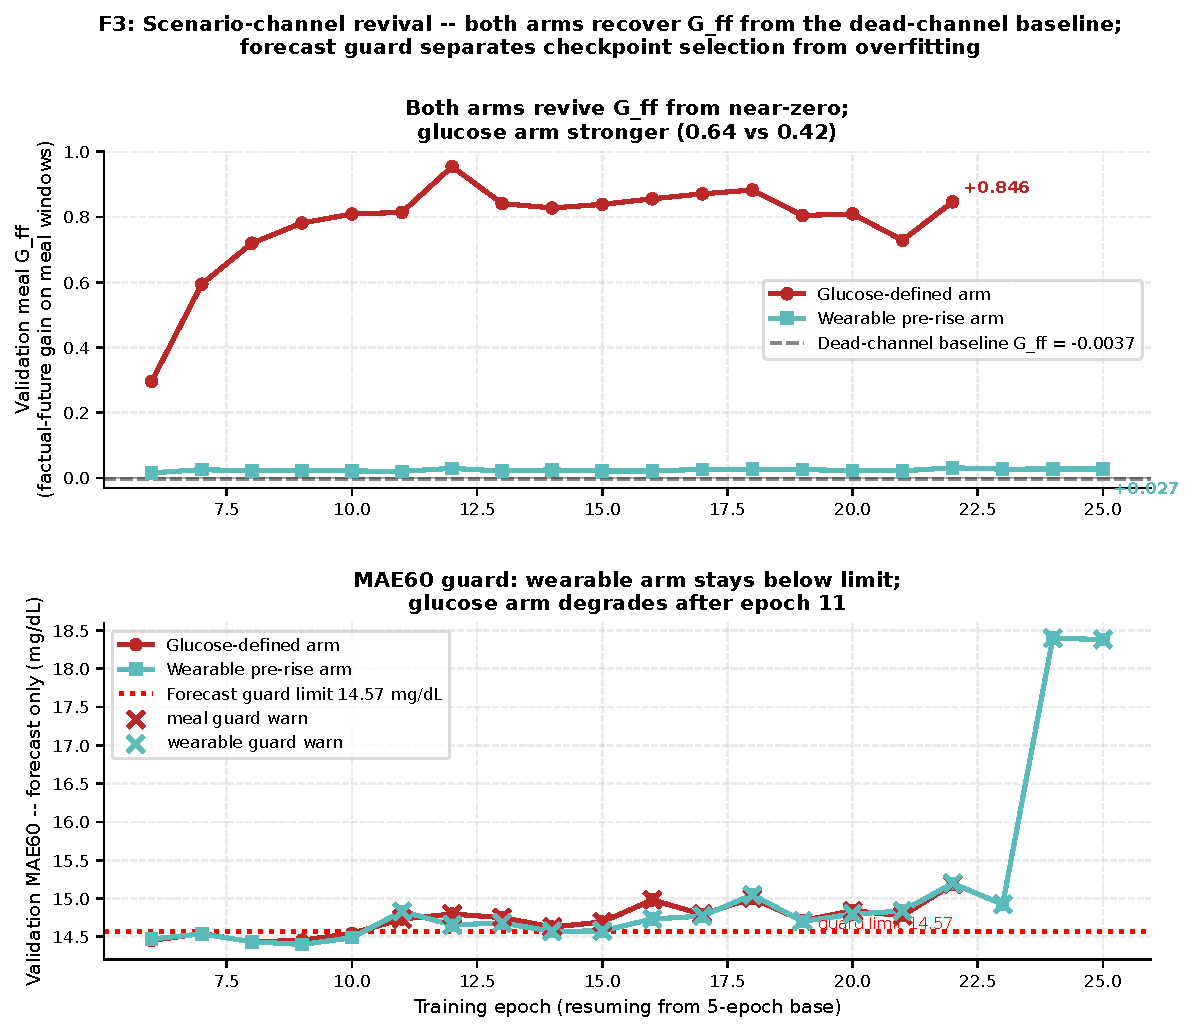
\includegraphics[width=\textwidth]{figures/meal_flags/f3_channel_revival.pdf}
    \caption{F3: Scenario-channel revival across both arms. \textbf{Top:} Validation meal $G_{\mathrm{ff}}$ by epoch; both arms recover from the dead-channel baseline (dashed gray). Glucose arm (crimson) reaches $+0.64$, wearable arm (teal) reaches $+0.42$ at epoch 8. \textbf{Bottom:} Validation MAE60 forecast-only guard; wearable arm stays below the limit; glucose arm exceeds it after epoch 11, confirming epoch 8 as the selected checkpoint for both.}
    \label{fig:f3_channel_revival}
\end{figure}

We then compared model implied counterfactual effects with matched observed meal-associated episodes. The observed natural-experiment effect was positive: glucose increased by about 22 mg/dL at 60 minutes. A valid meal counterfactual should at least match this direction.

The glucose defined arm failed this test. Its predicted effect was strongly negative, around -35 mg/dL at 60 minutes, while the observed matched effect was strongly positive. This suggests that the model learned a mean reversion or post rise correction pattern rather than the causal effect of eating.

The wearable arm did not show the same strong inversion, but its effect was near zero and slightly negative. Increasing the wearable scenario dose to match the model-space scale of the glucose-defined arm made the effect more negative, not positive. This rules out simple under-dosing as the explanation.(Fig.~\ref{fig:f4_cf_ab_headline})


\begin{figure}[h!]
    \centering
    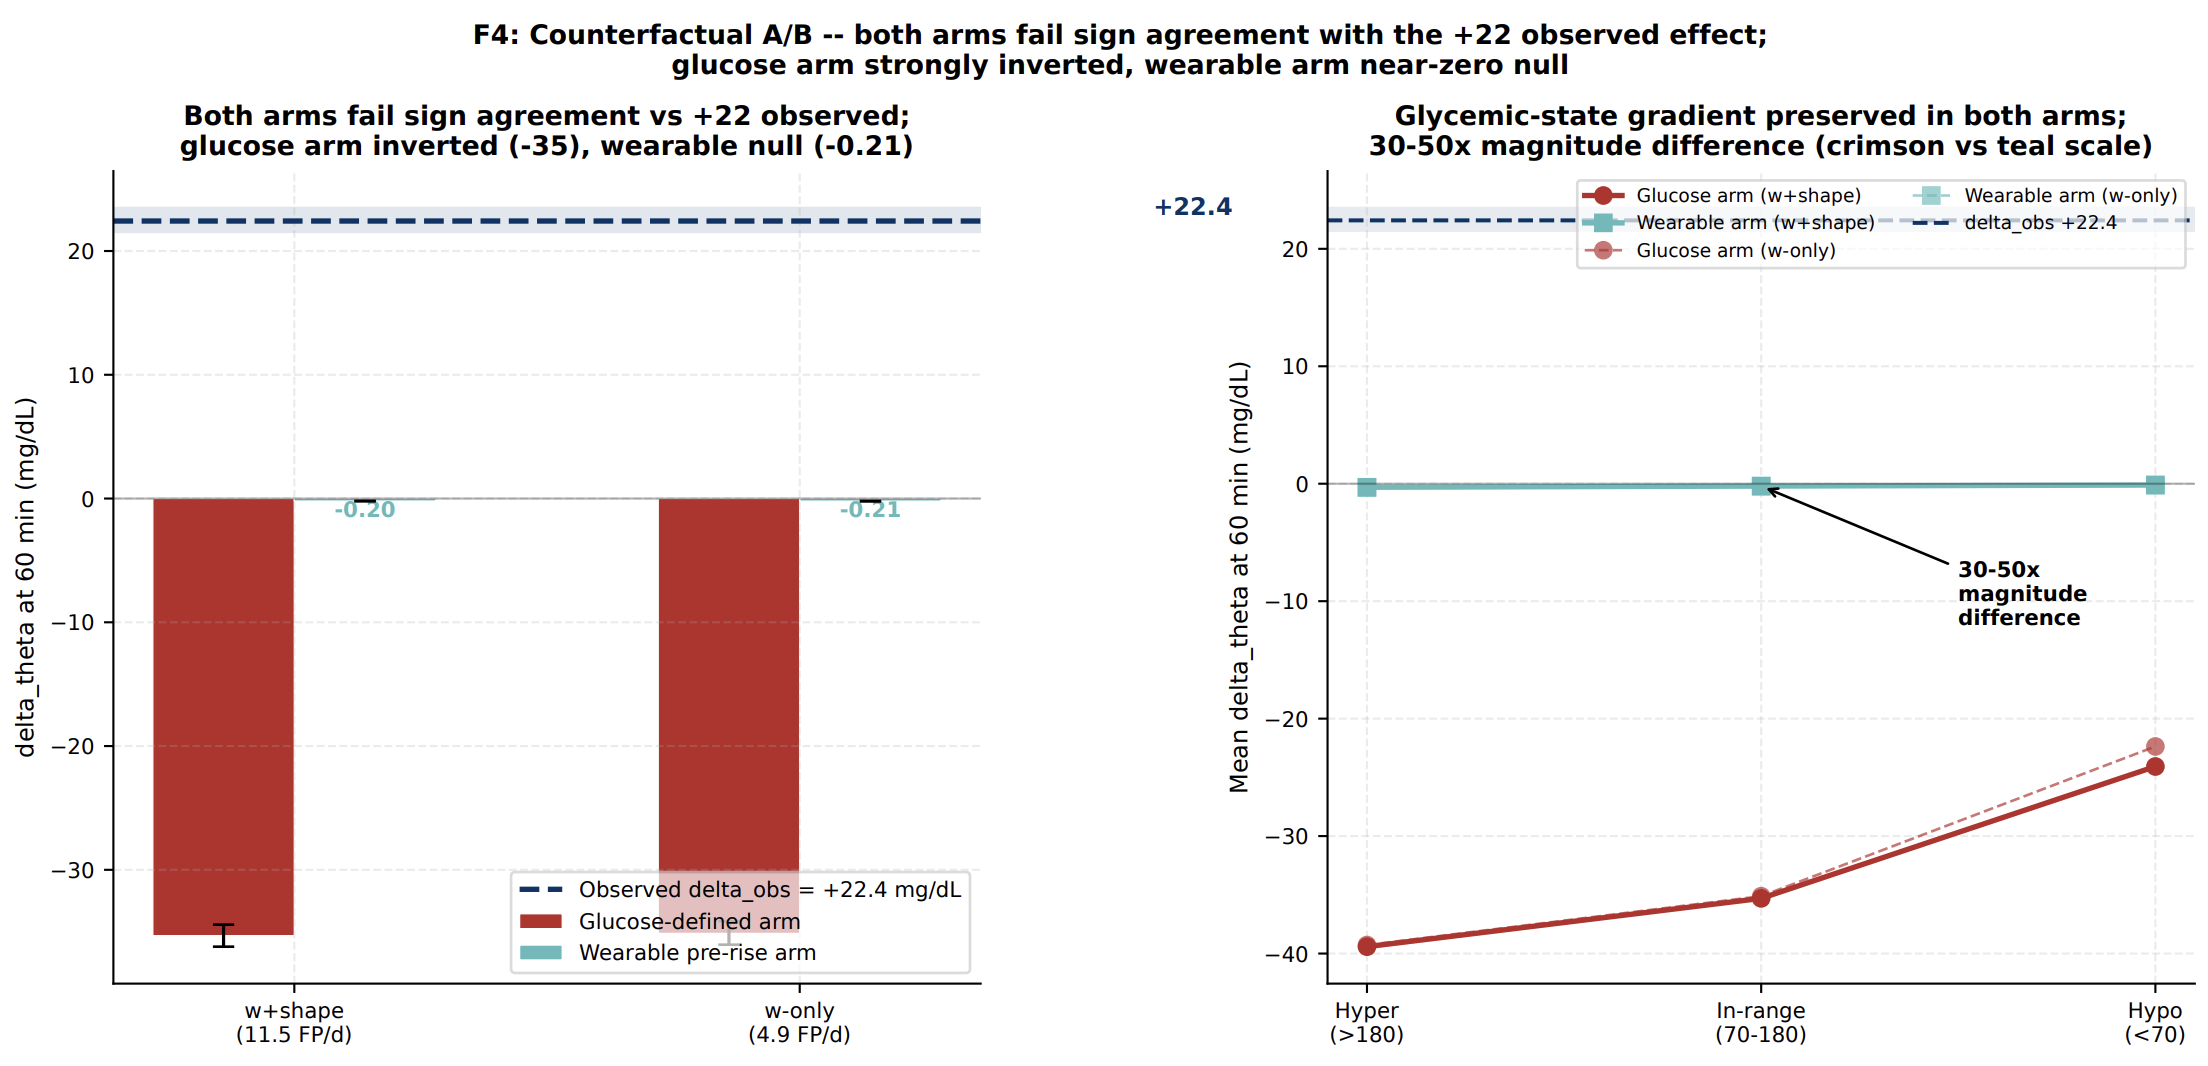
\includegraphics[width=\textwidth]{figures/meal_flags/f4_cf_ab_headline2.png}
    \caption{F4: Counterfactual A/B headline. \textbf{Left:} $\Delta\theta_{60}$ at both operating points; glucose arm (crimson) is strongly inverted at approximately $-35$ mg/dL, wearable arm (teal) is near-zero null at approximately $-0.21$ mg/dL; both fail sign agreement with the observed $+22.2$ mg/dL (navy dashed). \textbf{Right:} Glycemic-state gradient; the ordering is preserved in both arms but the magnitude differs by 30 to 50x (y-axis scales differ).}
    \label{fig:f4_cf_ab_headline}
\end{figure}

\begin{figure}[h!]
    \centering
    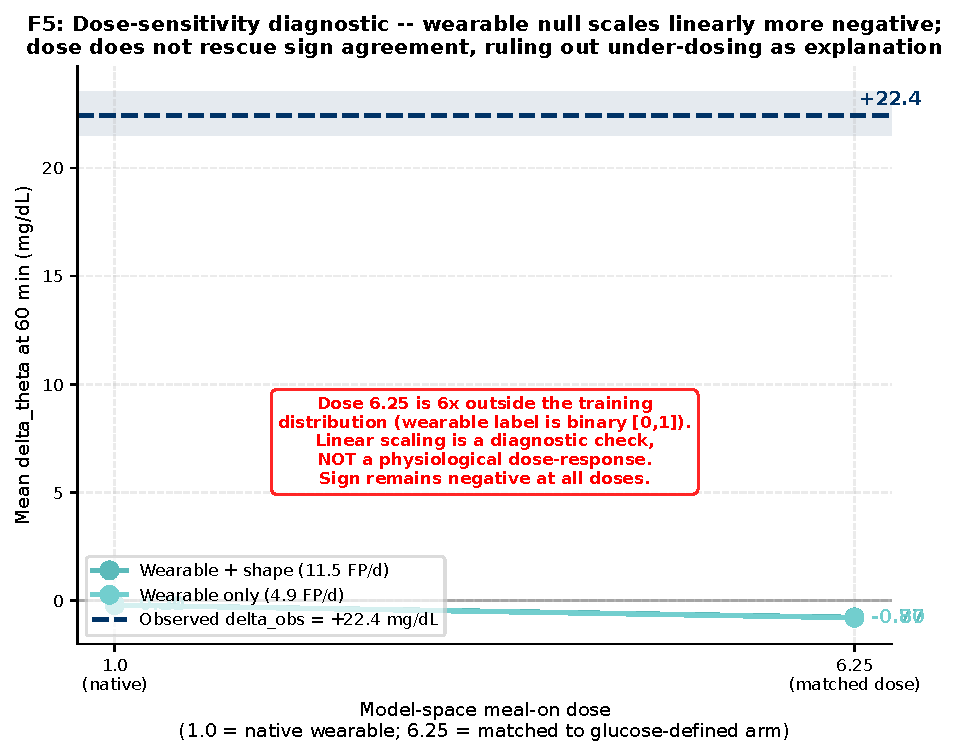
\includegraphics[width=0.65\textwidth]{figures/meal_flags/f5_dose_sensitivity.pdf}
    \caption{F5: Dose-sensitivity diagnostic. Wearable-arm $\Delta\theta_{60}$ at native model-space dose 1.0 and at dose 6.25 (matched to glucose-defined arm). Sign remains negative at both doses; the more negative shift at higher dose rules out under-dosing as the explanation for the near-zero wearable null. Dose 6.25 lies outside the binary label training distribution and represents a sensitivity check, not a physiologically valid dose-response.}
    \label{fig:f5_dose_sensitivity}
\end{figure}

The conclusion is therefore clear. Scenario aware retraining can make the counterfactual channel responsive, but the current AI-READI proxy labels do not yet produce a valid meal counterfactual. The model either learns the wrong direction from glucose defined labels or learns almost no usable effect from wearable labels. This supports the need for either stronger scenario supervision, explicit natural experiment agreement during training, or external datasets with real meal logs.

% =========================================================
\section{Study 1: Meal Counterfactual Audit}
\label{sec:study1_cf_audit}
% =========================================================

This section collects the complete artifact-grounded evidence summary for the meal counterfactual audit. All values in figures and tables are read from CSV artifacts and cross-checked at generation time. No values are hard-coded in prose or scripts without a corresponding CSV row.

\subsection{Leakage and Redundancy}
\label{subsec:study1_leakage}

Figure~\ref{fig:f1_leakage_redundancy} and Table~\ref{tab:t1_ablation} report the seven-setup ablation. The central empirical result is Eq.~\eqref{eq:meal-central-comparison}: $C \gg C' \approx D \approx H \approx A'$. The leakage-free causal teacher C' sits at the slope-and-clock baseline A', while the bidirectional teacher C reaches substantially lower MAE and peak error, but that gap is future-glucose leakage and is fully unreachable at deployment. The partial correlation of the deployable student D with the q50 residual after removing slope, level, and clock is 0.101, compared to 0.519 for the leaky teacher C and 0.027 for the causal ceiling C'. The near-collapse of causal partial correlations confirms that the deployable features carry little information orthogonal to the CGM slope already available in the base model.

\begin{figure}[H]
    \centering
    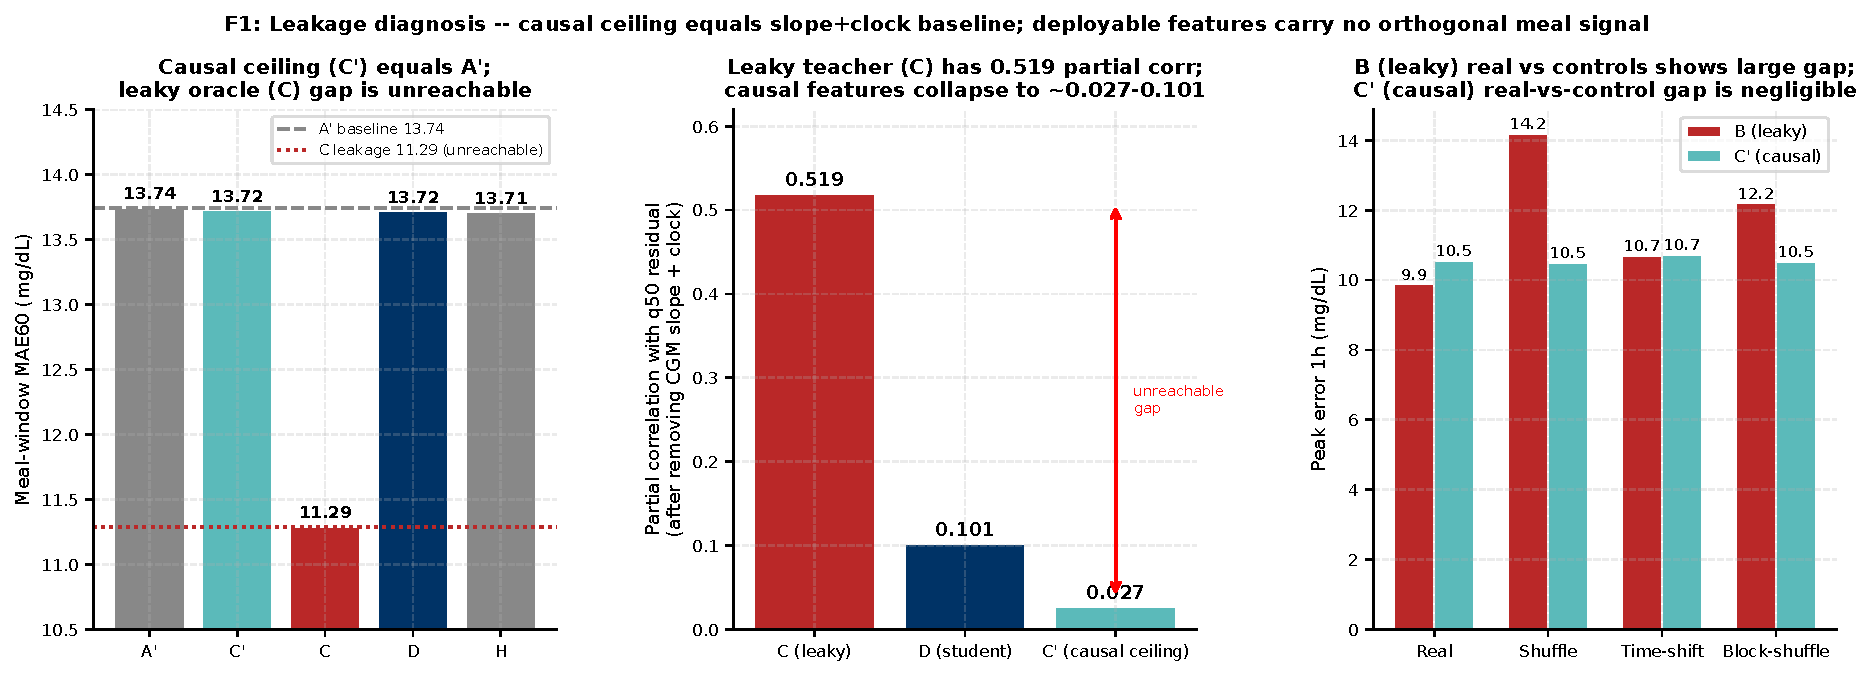
\includegraphics[width=\textwidth]{figures/meal_flags/f1_leakage_redundancy.pdf}
    \caption{F1: Leakage and redundancy diagnosis. \textbf{Left:} Meal-window MAE for key setups; the causal ceiling C' equals the slope-and-clock baseline A'; the leaky oracle C gap (dashed crimson) is unreachable. \textbf{Center:} Partial correlation with q50 residual after removing slope, level, and clock; only the leaky teacher C (0.519) carries substantial orthogonal signal. \textbf{Right:} Negative controls for B (leaky) and C' (causal) on peak error; B shows a large real-versus-control gap consistent with bidirectional access to future glucose; C' does not.}
    \label{fig:f1_leakage_redundancy}
\end{figure}

\begin{table}[H]
\centering
\footnotesize
\renewcommand{\arraystretch}{1.3}
\caption{T1: Seven-setup ablation on the non-insulin cohort. MAE values in mg/dL. Partial correlation is with the q50 residual after partialing out CGM slope, level, and clock. ``Leaky'' marks setups that read future glucose or future wearables at the anchor. Dashes indicate no partial-correlation test was run for the baseline setups.}
\label{tab:t1_ablation}
\setlength{\tabcolsep}{5pt}
\begin{tabular}{@{}lllcccc@{}}
\toprule
Setup & Label & Feature added & Leaky & MAE60 & Meal-wdw MAE & Partial corr \\
\midrule
q50 uncorrected & Baseline & None (pretrained q50) & No & 14.36 & 13.86 & -- \\
A' & Slope+clock & CGM slope and clock & No & 14.35 & 13.74 & -- \\
B & Old predmeal & Binary predmeal flag (bidir) & Yes & 13.74 & 13.23 & 0.278 \\
C & Bidir teacher & Continuous bidir teacher prob & Yes & 11.79 & 11.29 & 0.519 \\
C' & Causal teacher & Causal teacher prob & No & 14.33 & 13.72 & 0.027 \\
D & Student prob & Causal student probability & No & 14.31 & 13.72 & 0.101 \\
G & Online state & Online decoded meal state & No & 14.30 & 13.71 & 0.101 \\
H & Online full & Online state + phase decoder & No & 14.28 & 13.71 & 0.101 \\
\bottomrule
\multicolumn{7}{@{}l}{\footnotesize Source: \texttt{block3\_meal\_feature\_endpoints.csv} (non\_insulin cohort),
  \texttt{block3\_partial\_information.csv}.}
\end{tabular}
\end{table}

\subsection{Pre-Rise Detection Performance}
\label{subsec:study1_prerise}

The pre-rise wearable detector evaluation is summarized in Fig.~\ref{fig:f2_prerise_detector}. The key metric is detection latency relative to CGM-defined onset: the CGM-only baselines fire 35--40 min post-onset, well above the Hochsmann et al.\ 37-min wall; the wearable feature sets fire at 0--15 min median, with \texttt{wearable\_plus\_shape} achieving a 0-min median (46.8\% of detections are pre-rise, sensitivity 0.81) at the cost of 11.5 FP/day. This confirms the detector breaks the CGM-only wall, motivating its use as the anchor-selection operating point for the Block 3 evaluation.

\begin{figure}[H]
    \centering
    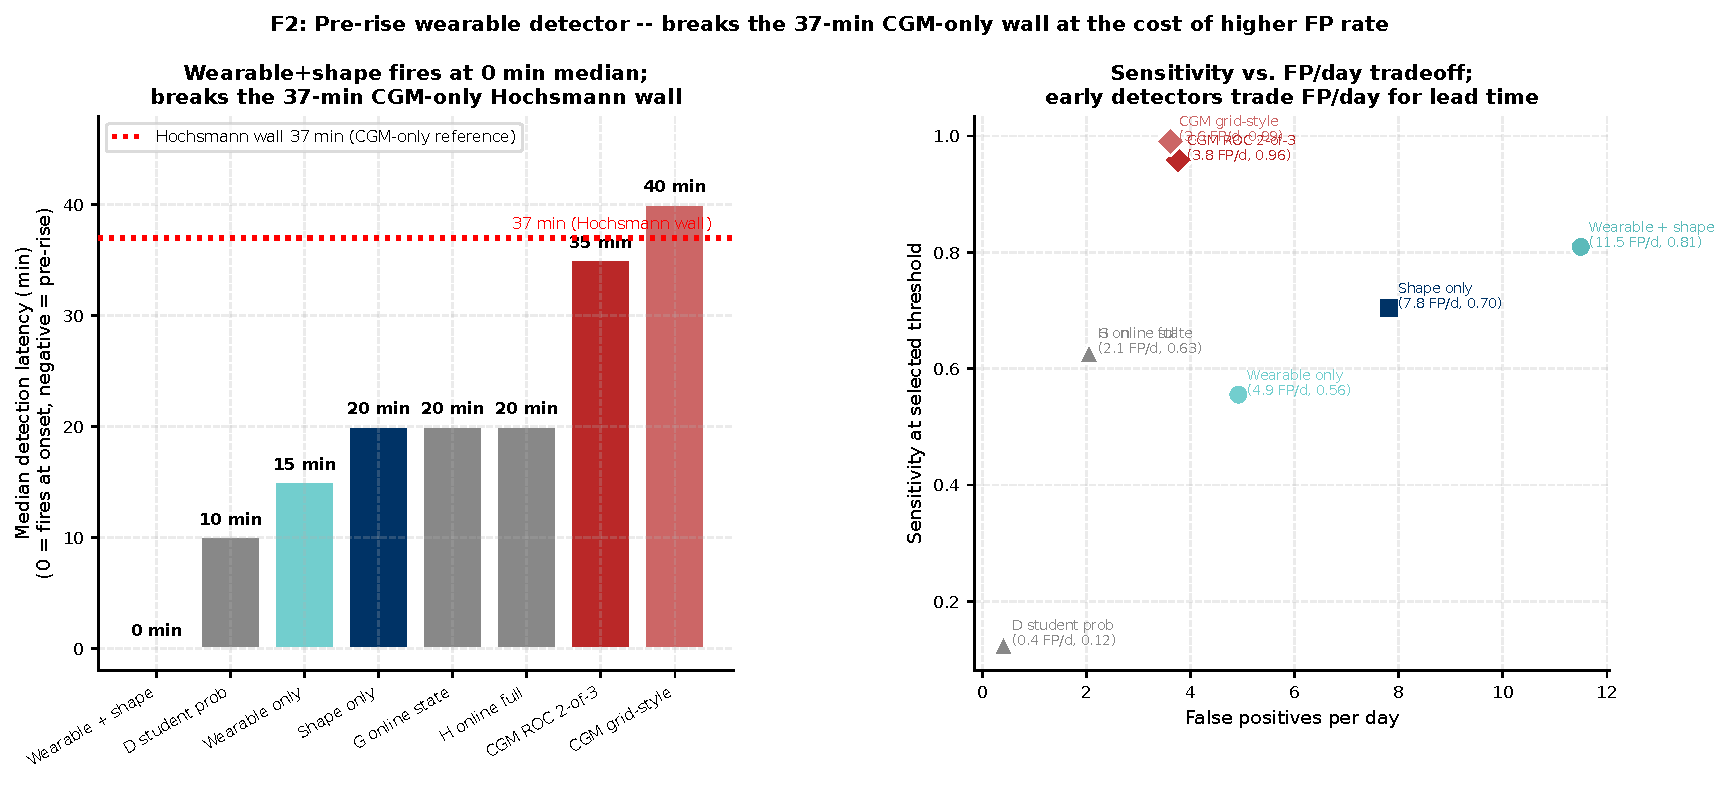
\includegraphics[width=\textwidth]{figures/meal_flags/f2_prerise_detector.pdf}
    \caption{F2: Pre-rise wearable detector. \textbf{Left:} Median detection latency by setup; dotted red line marks the Hochsmann et al.\ 37-min CGM-only reference. Wearable sets (teal) fire at 0--15 min; CGM baselines (crimson diamonds) at 35--40 min. \textbf{Right:} Sensitivity vs.\ FP/day tradeoff; early detection of meal onset requires accepting a higher false-positive rate.}
    \label{fig:f2_prerise_detector}
\end{figure}

\subsection{Evidence Boundary and Conclusions}
\label{subsec:study1_boundary}

Table~\ref{tab:t2_block3} and Fig.~\ref{fig:f6_summary_schematic} summarize the Block 3 results. Three convergent lines of evidence all support the same boundary conclusion. First, the orthogonalization audit (Section~\ref{subsec:study1_leakage}) shows that deployable features carry no meal-specific signal orthogonal to the CGM slope, ruling out any headroom from better feature engineering. Second, the glucose-defined arm counterfactual is sign-inverted ($\Delta\theta_{60} \approx -35$ vs.\ observed $+22.2$ mg/dL).The matched observed episodes show a positive glucose rise after meal associated events, while the model-implied glucose-defined scenario produces a large negative effect. This indicates that the model has not learned “meal causes glucose to rise.” Instead, it appears to have learned a post-rise correction or mean-reversion pattern. Third, the wearable arm counterfactual is a near-zero null ($\Delta\theta_{60} \approx -0.21$). Increasing the scenario dose does not fix the sign. Therefore, the problem is not simply that the wearable signal was too small; the current scenario channel still does not encode a physiologically valid meal effect. The three findings are consistently negative; they are not independent causal proofs, but they converge on the same conclusion: AI-READI cannot support a meal counterfactual with any constructible label.

\begin{table}[H]
\centering
\footnotesize
\renewcommand{\arraystretch}{1.3}
\caption{T2: Two-arm Block 3 counterfactual evaluation at 60 min horizon on the non-insulin cohort ($n = 200$ participants). $\Delta\theta_{60}$: model-implied meal-on minus forecast-only median; 95\% CI from participant bootstrap ($B = 1000$). $\Delta_{\mathrm{obs}} = +22.2$ mg/dL (95\% CI: 21.6 to 22.8) from matched natural experiment. Sign agreement column indicates whether $\Delta\theta$ and $\Delta_{\mathrm{obs}}$ share the same sign. Dose-matched rows use model-space 6.25 for the wearable arm (outside $[0,1]$ training distribution; diagnostic only).}
\label{tab:t2_block3}
\setlength{\tabcolsep}{4pt}
\begin{tabular}{@{}llrrrrrc@{}}
\toprule
Arm & Operating point & Dose & $\Delta\theta_{60}$ & 95\% CI & Anchors & Participants & Sign agree \\
\midrule
\multicolumn{8}{@{}l}{\textit{Glucose-defined arm (model-space 6.25 from preprocessor transform)}} \\
Glucose-def & \texttt{wearable\_plus\_shape} & 6.25 & $-35.3$ & $[-36.2,\ -34.4]$ & 6592 & 200 & No \\
Glucose-def & \texttt{wearable\_only} & 6.25 & $-35.1$ & $[-36.1,\ -34.2]$ & 4547 & 200 & No \\
\midrule
\multicolumn{8}{@{}l}{\textit{Wearable pre-rise arm (native dose, model-space 1.0)}} \\
Wearable & \texttt{wearable\_plus\_shape} & 1.0 & $-0.205$ & $[-0.212,\ -0.197]$ & 6592 & 200 & No \\
Wearable & \texttt{wearable\_only} & 1.0 & $-0.212$ & $[-0.219,\ -0.204]$ & 4547 & 200 & No \\
\midrule
\multicolumn{8}{@{}l}{\textit{Wearable arm (dose-matched to glucose-defined arm; sensitivity diagnostic only)}} \\
Wearable (dose-match) & \texttt{wearable\_plus\_shape} & 6.25 & $-0.775$ & $[-0.801,\ -0.747]$ & 6592 & 200 & No \\
Wearable (dose-match) & \texttt{wearable\_only} & 6.25 & $-0.798$ & $[-0.825,\ -0.771]$ & 4547 & 200 & No \\
\midrule
\multicolumn{8}{@{}l}{\textit{Glycemic-state gradient at \texttt{wearable\_plus\_shape} (glucose arm derived / wearable arm native)}} \\
Glucose-def & Hyper ($>180$ mg/dL) & 6.25 & $-39.4$ & $[-42.8,\ -36.4]$ & 255 & 41 & No \\
Glucose-def & In-range (70--180) & 6.25 & $-35.3$ & $[-36.2,\ -34.4]$ & 6256 & 199 & No \\
Glucose-def & Hypo ($<70$ mg/dL) & 6.25 & $-24.1$ & $[-29.9,\ -19.8]$ & 81 & 25 & No \\
Wearable & Hyper ($>180$ mg/dL) & 1.0 & $-0.303$ & -- & 255 & 41 & No \\
Wearable & In-range (70--180) & 1.0 & $-0.202$ & -- & 6256 & 199 & No \\
Wearable & Hypo ($<70$ mg/dL) & 1.0 & $-0.114$ & -- & 81 & 25 & No \\
\bottomrule
\multicolumn{8}{@{}l}{\footnotesize Sources: \texttt{block3\_60min\_operating\_point\_comparison.csv} (both arms),
  \texttt{block3\_60min\_glycemic\_state\_breakdown\_derived.csv} (glucose arm),}\\
\multicolumn{8}{@{}l}{\footnotesize \texttt{block3\_60min\_glycemic\_state\_breakdown.csv} (wearable arm),
  \texttt{natural\_experiment\_effects.csv}.}
\end{tabular}
\end{table}

\begin{figure}[H]
    \centering
    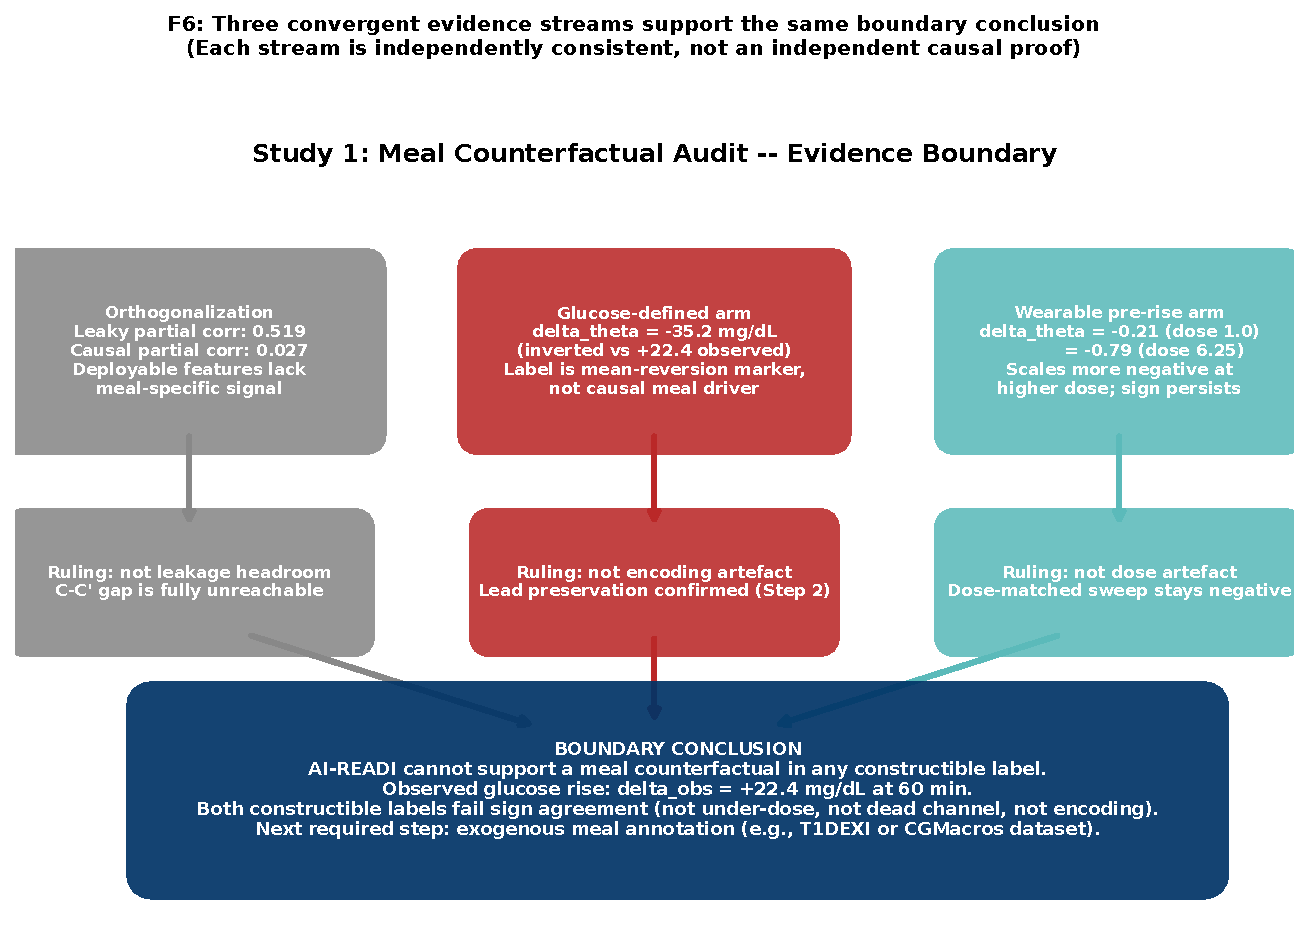
\includegraphics[width=0.8\textwidth]{figures/meal_flags/f6_summary_schematic.pdf}
    \caption{F6: Three convergent evidence streams supporting the boundary conclusion. Each stream rules out one alternative explanation (leakage headroom, encoding artefact, dose artefact), and all three converge on the same verdict. The streams are independently consistent; they are not independent causal proofs. The boundary conclusion follows from their convergence, not from any single test.}
    \label{fig:f6_summary_schematic}
\end{figure}

\paragraph{Boundary conclusion.}
AI-READI cannot support a meal counterfactual in any constructible label given the current dataset. The observed glucose rise is $\Delta_{\mathrm{obs}} = +22.2$ mg/dL at 60 min. Both constructible labels fail sign agreement at every dose and every operating point. The failure is not attributable to dead channels (G\textsubscript{ff} was successfully revived), dose magnitude (dose-matched sweep confirms), or encoding artefacts (lead preservation was confirmed in Step 2). The required next step is exogenous meal annotation from a dataset with prospective logging (for example, T1DEXI or CGMacros), which would enable a label that carries pre-rise causal information not derivable from the CGM slope alone.

\subsection{Study Framing}
\label{subsec:study_framing}

This report presents one of three planned studies.

\textbf{Study 1: Meal Counterfactual Audit} (this section). Concludes that AI-READI does not support a meal counterfactual with any constructible label. The boundary is established by three convergent checks: orthogonalization, glucose-defined arm inversion, and wearable arm dose-scaled null. The recommended next step is evaluation on a dataset with exogenous meal annotations.

\textbf{Study 2: Insulin and Medication Counterfactuals.} Asks whether the scenario-aware channel supports a valid insulin-dose or medication-adherence counterfactual on AI-READI, where external covariates provide labeling that does not depend on the CGM slope. The insulin quarantine and the low-confidence medication flags established in this report define the scope of that evaluation.

\textbf{Study 3: Downstream Clinical Decision Support.} Asks whether the SSM-CGM streaming distribution, with or without a valid counterfactual channel, supports reliable hyperglycemia or hypoglycemia risk alerts at the operating points identified by the pre-rise detector. This study uses the hyperglycemia AUPRC and recall endpoints already reported in Table~\ref{tab:t1_ablation} as its primary metrics.
